\section{Secret, Arcanum, Mystery}

\begin{wrapfigure}{rt}{.3\textwidth}
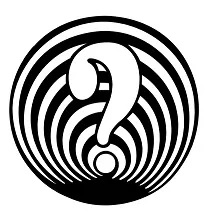
\includegraphics[width=.25\textwidth]{Mystery.jpg}
\end{wrapfigure}

Hermetism distinguishes between three closely related words:

\begin{itemize}


\item Secretum (secret)

\item Mysterium (mystery)

\item Arcanum
\end{itemize}


It is important to keep these distinctions in mind.

\paragraph{Secret}


A secret is a fact, procedure, practice, or doctrine which a number of men agree to hide. There is no inner transformation required to know a secret. I can tell you where the treasure is buried; you can then find it and remain the same person you were before. A secret is hidden in the darkness.

\paragraph{Mystery}


A mystery, in contrast, is hidden in the light. According to Tomberg:

\begin{quotex} 
A mystery is a spiritual event comparable to physical birth or death. It is a change of the entire spiritual and psychic motivation, or a complete change of the plane of consciousness.
\end{quotex}


There are those who tell me that an intelligent man does not believe in miracles. Yet that same man is not at all concerned about why there is such a being as an intelligent man in the first place. To understand that requires unveiling a mystery.

\paragraph{Arcanum}


An arcanum, on the other hand, is hidden in the twilight. They may be symbols, myths, or rituals that both conceal and reveal their meaning, depending on the depth of meditation or understanding. To the uninitiated, an arcanum will be interpreted as an allegory, or even nonsense; he cannot be simply told the meaning, as though it were a mere secret. But to the initiate, an arcanum reveals

\begin{quotex}
that which is necessary to know in order to be fruitful in a given domain of spiritual life. It is that which must be actively present in our consciousness---or even in our subconscious---in order to render us capable of making discoveries, engendering new ideas, conceiving new artistic subjects. In a word, it makes us \emph{fertile} in our creative pursuits, in whatever domain of spiritual life. An arcanum is a ferment or an enzyme whose presence stimulates the spiritual and the psychic life of man. And it is symbols which are the bearers of these ferments or enzymes and which communicate them---if the mentality and morality of the recipient is ready.
\end{quotex}



\flrightit{Posted on 2010-10-25 by Cologero}

\begin{center}* * *\end{center}

\begin{footnotesize}
\begin{sffamily}
\texttt{James O'Meara on 2010-10-26 at 14:02 said:}

`` A mystery is a spiritual event comparable to physical birth or death. It is a change of the entire spiritual and psychic motivation, or a complete change of the plane of consciousness.''

As Aristotle observed, one participated in the Mysteries not to acquire knowledge but to undergoe an experience, viz, a transfomation.

\end{sffamily}
\end{footnotesize}

